
\chapter{Object definitions}
\label{ch:objects}
%\epigraphfontsize{\small\itshape}
\epigraph{\itshape``All compromise is based on give and take, but there can be no give and take on fundamentals. Any compromise on mere fundamentals is a surrender. For it is all give and no take. }{--- \textup{Mahatma Gandhi}}

\normallinespacing
\mediumlinespacing

\section{Introduction}


\hspace{10pt} The foundation of most experimental studies is based around the connection between the original idea and the actual reality presented in the form of technical possibilities, in practice more likely limitations, given by the apparatus at hand. The same statement is applicable for the main interest of this thesis. The idea is very appealing on paper (as previously discussed in Chapter~\ref{ch:Higgs_LHC_DM}), there is a production mode with a strong signature and a possible decay that is highly suppressed when looked at from the SM point of view.

\hspace{10pt} From the perspective of the CMS experiment, each analysis needs to be built from the ground up using the same basis - reconstructed physics objects. Following the conclusion that a good way to describe the "invisible" part of an event is through the usage of the $E_{T}^{miss}$ and through its definition in Equation~\ref{for:met}, it can be seen that it takes the collective information from all parts of the detector to quantify the possible invisible contribution. Speaking in technical terms, all available objects will have a role to play in this analysis. This chapter will serves as a summary of the processes and algorithms used in order to reconstruct and define the base objects used in physics analyses.% Taking into account that this study covers different eras of the Run-2 phase of the LHC, each object will be defined separately for every year of data taking to accommodate for different conditions of the CMS detector during where necessary.

\section{Particle Flow reconstruction}
\label{sec:particle_flow}
\hspace{10pt} With the limitations imposed by a large stream of events being removed through the usage of a two level triggering system, more detailed reconstruction can be used for the full (offline) reconstruction of physics objects. The PF algorithm~\cite{Particle_flow,CMS-PAS-PFT-09-001,PF:Florian} provides a valuable tool that connects information originating from all detector subsystems in order to provide the most detailed overview of the event possible. It relies on the features of the CMS detector to deliver exceptional tracking performance which is then combined with the information coming from calorimeters and muon detectors. The idea of combining calorimeter crystals into TTs replaced with the plan to identify, as precisely as possible, all stable particles originating from collision interactions, hence giving rise to PF candidates. The subsequent grouping of those PF candidates and performing identification techniques, as well as energy sum computations, provides analysers with a set of object collections on which to build their analysis on.


\hspace{10pt} In order to efficiently present object collections vital to the main study of this thesis, each of the following sections will provide a brief overview of the reconstruction techniques used to define a particle collection. This description will be followed by a set of recommendations given by the corresponding CMS Physics Object Group (POG), which are then used to create separate collections for a particle type used further down the analysis chain (i.e. formation of the dedicated control regions etc.).


\subsection{Tracks and Primary Vertex}
\label{sec:tracking}
\hspace{10pt} The tracker information on charged particles is essential in their further identification and usage. The tracker also imposes itself as a better solution when measuring the momenta of charged hadrons than calorimeters (due to the energy loss in material before reaching them) with the added bonus of being able to pinpoint the original directions of particles before being affected by the magnetic field. This all indicates that the preferred course of action is to have the tracking efficiency being as high as possible~\cite{PF:track}. In order to achieve that, an iterative approach is deployed.

\hspace{10pt} A set of tightly tailored requirements is imposed in order to select a first set of tracks. This ensures the purity of track through the removal of fake contributions. The downside of this choice, the lack of high efficiency in track reconstruction, can be eliminated with next steps. The preparation for the second iteration sees the removal of high purity tracks selected in the first step while partially loosening the tight restrictions imposed on track candidates. This approach yields an increase in efficiency while keeping the high purity of selected tracks. A slight change in the approach is introduced after the third iteration. The last two iteration steps are responsible for covering particles originating from secondary vertices, which is being enabled through a modification of requirements regarding the track's origin.

\hspace{10pt} Finally, in order to conclude this discussion, a choice of a primary vertex needs to be made. This is done by looking at the sum of $p_T^2$, where the sum goes over all reconstructed tracks. The vertex with the largest value is chosen to be the primary vertex for the event.

\subsection{Muons}
\label{subsec:muons}
%The basis used to define muons is the \emph{Muon} collection obtained from the nanoAOD trees. As with the \emph{Electron} objects, this collection is centrally produced.

\hspace{10pt} The easiest way to start discussing the definition of muons is to take a look at the criteria helping with the definition of loose muon objects (in further text referred to as Loose Muon ID). This categorisation is important in order to increase the purity of muon objects throught the removal of contributions originating from charged hadrons. When applied to a PF object%~\footnote{In this case "Reco Muons", which can contain additional contributions arising from charged hadrons that have beed missed in the identification process}
, the Loose Muon ID requires fulfilment of a few quality conditions. First, the object being looked at needs to be reconstructed as a PF Muon, accompanied by a supplementary condition that this PF Muon candidate needs to be defined either as a Global or a Tracker Muon~\cite{paper:pf_muon_1,paper:pf_muon_2}. 

\hspace{10pt} Both of the aforementioned requirements look for the scenario where the information about the muon candidate's track (originating from the muon subsystems) has been matched to its tracker counterpart. For the Global Muon criteria, tracks originating from two centres of information are extrapolated onto the same plane, upon which respective companions are being selected (one from each set). From there, a global track is extracted via a combined, Kalman-filter approach~\cite{pf:kalman}, fit using the information coming from, previously paired, tracks. The Tracker Muon criteria takes a slightly different approach. It considers all particles which pass very loose conditions\footnote{$p_T>$0.5~GeV and $p>$2.5~GeV} and extrapolates their tracks to the muon detectors while taking into account detector effects. If a hit in muon detectors can be associated with one of these tracks, the PF candidate is considered to be a Tracker Muon.

\hspace{10pt} Following the blueprint instructed by the Muon POG~\cite{muon_pog_1}, the definition of a tight muon objects imposes a stricter requirement on candidates by requiring the object to be a Global Muon with additional quality requirements (in further text referred to as Tight Muon ID). The first pair of quality requirements asks for a goodness of fit for the global muon track be expressed through $\chi^2/N_{DoF}<$~10 and the inclusion of at least one muon chamber hit (with there being at least two) in the aforementioned fit in order to suppress the fake contribution. Further suppression of these effects is enabled through the usage of $d_{xy}<$~2~mm, $d_z<$~5~mm~\footnote{Representing the transverse impact parameter and the z-axis distance of the track when taking the primary vertex as the point of origin} and $N^{hits}_{pixel}>$~0. Finally, in order to achieve an accurate measurement of muon $p_T$, a $N_{tracker}^{hits}>$~5 requirement is imposed. 

\hspace{10pt} Speaking in terms of the analysis level objects, previously defined Loose and Tight Muon ID criteria are combined with additional kinematic ($p_T>$~10/20~GeV), geometric ($|\eta|<$~2.4) and isolation ($\text{I}_{\Delta R<0.4}^{Rel.}<$~0.25/0.15\footnote{The relative isolation variable is defined as the ratio of the sum of $E_T$ of photons and $p_T$ of charged hadrons with respect to the muon candidate’s $p_T$ (where the sum covers particle candidates over the area of $\Delta R<0.4$).}) requirements in order to form the Loose and Tight Muon collections (respectively).

%\begin{table}[htbp]
%\centering
%\caption{Requirements used to define the Loose Muon collection\label{tab:loosemuon}}
%\begin{tabular}{l|c}
%\hline\hline
%Requirement   & Definition                                                          \\ \hline
%$|\eta| < 2.4$ & -                                                                    \\
%$p_{T} > 10~GeV$     & -                                                                    \\
%\texttt{looseId} $= 1$  & Loose Muon ID \\
%$\text{I}_{\Delta R<0.4}^{Rel.}<$ 0.25 & PF relative isolation~\footnote{}  \\
%\hline\hline
%\end{tabular}
%\end{table}

%\begin{table}[htbp]
%\centering
%\caption{Requirements used to define the Tight Muon collection\label{tab:tightmuon}}
%\begin{tabular}{l|c}
%\hline\hline
%Requirement    & Definition                                                          \\ \hline
%\text{LooseMuon requirements} &                                                                     \\
%\texttt{tightId} $= 1$     & Tight Muon ID\\             
%$\text{I}_{\Delta R<0.4}^{Rel.}<$0.15 & PF relative isolation           \\ \hline\hline
%\end{tabular}
%\end{table}




\subsection{Electrons}
\label{subsec:electrons}
\hspace{10pt} The interaction of electrons with the tracker material can lead to Bremsstrahlung radiation manifesting itself in the form of emitted photons. Other detector effects such as the strong magnetic field cause electron energy deposits to be spread out in the $\phi$ range of ECAL~\cite{paper:pf_muon_1,note_ele_reco,twiki_egamma_1}. %Depending on the value of the particle's transverse momenta, two approaches can be taken in order to reconstruct electrons.

\hspace{10pt} Taking a look at the information given by the calorimeter, it can be seen that $\sim$~97~\% of electron's energy (the same statement stands for photons) is deposited in a 5x5 ECAL crystal structure named the supercluster~\cite{twiki_ecal_clustering}. This allows for a matching procedure to be applied, pairing the supercluster to an electron track (obtained through a fit strategy which takes detector effects into account). As the transverse momenta goes down in value, it becomes more difficult to use the aforementioned approach due to the fact that the radii of the curvature of the particle's trajectory gets smaller. This introduces a problem for the supercluser formation as now the photon contribution (originating from Bremhsstrahlung) can be much further in $\phi$ than before, asking for a more careful approach using a multivariate estimator in order to discover pure electron tracks (being relevant for values of $p_T<$~10~GeV).

%The importance of electrons is best definition of the Signal Region requires a veto on the electron objects, while the formation of two out of four Control Regions asks for the existence of specific types of electrons in the event.
\hspace{10pt} Following recommendations given by the E/Gamma POG~\cite{twiki_egamma_1,twiki_egamma_2}, definitions of two main electron collections used in this analysis (Veto and Tight) are summarized in Tables~\ref{tab:electronIDb2017} and \ref{tab:electronIDe2017} (in further text referred to as Cut Based ID). Similarly to the previous section, which dealt with the definition of muon collections, when approaching the definition of analysis level electron collections, the POG recommended Veto and Tight ID criteria are combined with kinematic ($p_T>$~10/40~GeV), geometrical ($|\eta|<$~2.5) and impact parameter requirements\footnote{For the barrel section a requirement of $|d_{xy}|<$~0.05 and $d_z<$0.1 is imposed, while the endcap requirement asks for $|d_{xy}|<~$0.1 and $d_z<$~0.2} in order to acquire the final Veto/Tight Electron collection (respectively). 
\begin{table}[h]
\footnotesize
\centering
\begin{tabular}{|l|c|c|}
\hline\hline
Requirement    & Veto  & Tight             \\\hline
full 5x5 $\sigma_{i\eta i\eta}$ &  $< 0.0126$ &   $< 0.0104$    \\
$|\Delta\eta_{\mathrm{In,seed}}|$ & $< 0.00463$ & $< 0.00255$ \\
$|\Delta\phi_{\mathrm{In, seed}}|$ & $< 0.148$ & $< 0.022$ \\
H/E & $<$ 0.05+1.16/$E_{\mathrm{SC}}$+0.0324$\rho$/$E_{\mathrm{SC}}$ & $<$ 0.026+1.15/$E_{\mathrm{SC}}$+0.0324$\rho$/$E_{\mathrm{SC}}$ \\
Rel. Isolation With EA & $<$ 0.198+0.506/$p_T$	& $<$ 0.0287+0.506/$p_T$\\
$|1/\mathrm{E} - 1/\mathrm{p}|$ & $<$ 0.209	& $<$ 0.159\\
Exp. Missing Inner Hits & $\leq$ 2&	 $\leq$ 1\\
Pass conversion veto & yes	& yes \\
\hline\hline
\end{tabular}
\caption{Summary of E/Gamma POG recommendations used to define Veto and Tight electrons in the barrel region ($|i\eta|\leq 1.479$)~\cite{twiki_egamma_1,twiki_egamma_2,note:AN_19_257}. The conventional names $|\Delta\eta_{\mathrm{In,seed}}|$ and $|\Delta\phi_{\mathrm{In,seed}}|$ represent the geometrical distance between the extrapolated electron track and the selected supercluster. The $\sigma_{i\eta i\eta}$ variable is used to quantify the $\eta$ dimension of the supercluser (weighted by its energy). Finally, the H/E variable controls the ratio of HCAL over ECAL contribution.}
\label{tab:electronIDb2017}
\end{table}

\begin{table}[h]
\footnotesize
\centering
\begin{tabular}{|l|c|c|}
\hline\hline
Requirement    & Veto  & Tight             \\\hline
full 5x5 $\sigma_{i\eta i\eta}$ &  $< 0.0457$ &   $< 0.0353$    \\
$|\Delta\eta_{seed}|$ & $< 0.00814$ & $< 0.00501$ \\
$|\Delta\phi_{in}|$ & $< 0.19$ & $< 0.0236$ \\
H/E & $<$ 0.05+2.54/$E_{SC}$+0.183$\rho$/$E_{SC}$ & $<$ 0.0188+2.06/$E_{SC}$+0.183$\rho$/$E_{SC}$ \\
Rel. Isolation With EA & $<$ 0.203+0.963/$p_T$	& $<$ 0.0445+0.963/$p_T$\\
$|$1/E-1/p$|$ & $<$ 0.132	& $<$ 0.0197\\
Exp. Missing Inner Hits & $\leq$ 3&	 $\leq$ 1\\
Pass conversion veto & yes	& yes \\
\hline\hline
\end{tabular}
\caption{Summary of E/Gamma POG recommendations used to define Veto and Tight electrons in the endcap region ($|i\eta|> 1.479$)~\cite{twiki_egamma_1,twiki_egamma_2,note:AN_19_257}. The naming convention used for control variables follows definitions introduced with Table~\ref{tab:electronIDb2017}. }
\label{tab:electronIDe2017}
\end{table}
\subsection{Photons}
\label{subsec:photons}
\hspace{10pt} Staying within the ECAL area of authority, the next item of discussion is the definition of the photon object collection. Upon completing definitions of collections revolving around charged particles and removing their contributions from the ECAL summary, the resulting clusters are used to form photon candidate objects. Further identification of candidates involves using algorithms which vary supercluster dimensions by using a set of predefined shapes associated with a photon deposit~\cite{note:AN_19_257,paper_photon_1} as well as relying on isolation variables. The definition of isolation requirements follows the idea that the scalar sum of transverse momenta of PF candidates (not being associated with the photon candidate's EM shower) is located around a certain geometrical distance from the tested object (in this case $\Delta R<$~0.3).

\hspace{10pt} Being used for vetoing in the process of reducible background rejection, the definition of photons for this analysis involves using objects which pass the Loose photon criteria provided by the E/Gamma POG~\cite{twiki_photon_1} (summarised in Table~\ref{tab:PhotonIDLoose}). Additional kinematic ($p_T>$~15~GeV) and geometric ($|\eta|<~$2.5) requirements are introduced alongside the Photon ID when defining the analysis level collection.


\begin{table}[htb!]
\centering
\footnotesize
%\def\arraystretch{1.2}
\begin{tabular}{l c}
\hline
Variable                                   &  Requirement: Barrel (Endcap)  \\
\hline
\hline
Full 5x5 $\sigma_{i\eta i\eta}$            & $< 0.0106 $ ($< 0.0272 $)    \\
H/E                                        & $<  0.04596 $ ($< 0.0590 $)    \\
charged hadron isolation                   & $< 1.694 $  ($< 2.089 $)     \\
neutral hadron isolation                   & $< 24.032 (19.722) + 0.01512(0.0117)\cdot p_T+2.259(2.3)\times 10^{-5} \cdot {p_T}^2$ \\
photon isolation                           & $< 2.876 (4.162) + 0.004017(0.0037)\cdot p_T$  \\
Conversion safe electron veto              & Yes (Yes)           \\
\hline
\end{tabular}
\caption{Requirements used to define loose photon objects~\cite{note:AN_19_257,twiki_photon_1}.}
\label{tab:PhotonIDLoose}
\end{table}




\subsection{Jets}
\label{sec:jets}
\hspace{10pt} Identification of jets is enabled through the use of the anti-$k_T$ algorithm~\cite{anti_kt}. It produces PF jet candidates which are then used as the basis for creating analysis level jet collections. The aforementioned algorithm, relies on the following properties when defining a jet:
\begin{equation}
    d_{i,B} = \frac{1}{p_{T_i}^2}
\end{equation}
\begin{equation}
    d_{i,j} = min\left (\frac{1}{p_{T_{i}}^2}, \frac{1}{p_{T_{j}}^2}\right )\frac{\Delta R_{i,j}^2}{R^2}
\end{equation}

where $p_{T_{i/j}}$ are transverse momenta of particles $i$ and $j$, $\Delta R_{i,j}$ is the geometrical distance between those particles. The $R$ parameter (taking the value of 0.4 in this scenario) is used as a benchmark jet cone size (similar to the choice of TTs when defining Level-1 jets in Section~\ref{l1:TTs})~\cite{note:AN_19_257}.  

\hspace{10pt} The algorithm compares candidates by taking a look at two properties forming the definition of $d_{i,j}$: the transverse momenta and geometrical distance. The scenario where $p_{T,i}>>p_{T,j}$ leads to the point that soft jet candidates will provide smaller values of $d_{i,j}$ as compared to situations where $p_{T_i}\sim p_{T_j}$. On the other hand, another comparison point is made through the geometrical search for particle's neighbours. If, for a selected hard jet candidate, there are no more high $p_T$ jets in the $\Delta R = 2R$ area, the algorithm will assign all soft jets found in $\Delta R_{i.j} = R$ area to this hard jet. For the scenario where there is another hard jet within the $2R$ area, another comparison of momenta is going to be deployed in order to create final jets\footnote{Another scenario may happen where there will be two hard jets within a $\Delta R_{i,j}< R$ area, which would require another comparison based on their respective $p_T$ values}. The creation of jet collection deploys an iterative approach through the usage of this algorithm, with the $d_{i,B}$ being used to compare the $p_T$ of jet objects created through the previously described process.

\hspace{10pt} Comparing the reconstructed jet $p_T$ values between data and simulation leads to the conclusion that the resulting $p_T$ value differs by $\sim 5-10~$\% from the true momenta (where the comparison is inclusive of the full detector acceptance and $p_T$ spectra)~\cite{note:AN_19_257}. Jet objects are corrected for the contribution originating from pileup through the introduction of an offset in their respective energies. These jet energy corrections are obtained from simulation~\cite{note:AN_19_257,paper_jes_jer,twiki_jes_jer}.

\hspace{10pt} Following recommendations given by the Jet/MET POG~\cite{twiki_jet_met} a set of quality criteria (Jet ID) are added on top of PF jet collection in order to create analysis level objects~\cite{twiki_jet_id}. These involve using a dedicated threshold on the fractions of neutral particles from ECAL and HCAL contributions as well as the muon fraction, number of constituents in a jet object, and the number of neutral particles. This study used the tight Jet ID working point, ensuring identification efficiency of $>99/98~$\% for 2017/2018 eras. Jet ID requirements are supplemented with a requirement of using a medium point of Jet Pileup ID in order to reject pileup contributions~\cite{twiki_jet_pileupid}. For the 2017 era of data taking, an additional veto requirement was added for jets within $p_T<$~50~GeV and $2.65<|\eta|<3.139$ range in order to suppress the contribution from jets originating from detector noise~\cite{note:AN_19_257}. This final collection is cleaned from overlap with the lepton and photon collection using a $\Delta R<~$0.4 condition.
\subsection{B jets}
\hspace{10pt} The definition of b jets\footnote{The b jets or beauty quark jets represent, as the alternative name suggests, jets originating from b quarks.} is important for the control of reducible SM background processes as these objects are used to veto events. This action is closely connected with the contributions originating from top quark processes~\cite{note:AN_19_257}. The POG recommended quality criteria advises the usage of the DeepCSV (Combined Secondary Vertex) tagging algorithm~\cite{paper_deepcsv} with a working point of 0.4941 and 0.4184 for 2017 and 2018 era respectively~\cite{twiki_btag_1}. These numbers correspond to a medium working point of DeepCSV algorithm ensuring an 80~\% efficiency of identifying a b jet. Additional kinematic ($p_T>$~20~GeV) and geometric ($|\eta|<$~2.4) requirements are applied when forming the analysis level object collection.
\subsection{Tau leptons}
\hspace{10pt} Similarly to the previous section, tau objects are important for vetoing events, thus reducing the contribution of V+jets SM backgrounds. A special algorithm is deployed in order to select the hadronically decaying taus\footnote{The final state particles originating from lepton decays of taus are already included in respective muon/electron collections.}. The idea behind the algorithm is to check if the jet object is comprised from objects associated with a tau decay. The selected tau candidates are requested to be completely isolated from other objects (the comparison point for the isolation is $\Delta R<$~0.5/0.3 for 2017/2018 era). Finally, a set of kinematic ($p_T>$~20~GeV) and geometric ($|\eta|<~$2.3) requirements is imposed when creating the analysis level collection~\cite{twiki_tau_pog}.

\subsection{Missing transverse energy}
\hspace{10pt} Defined with Equation~\ref{for:met}, the $E_{T,miss}$ variable provides an important view of the transverse contribution of particles invisible to the detector. From the reconstruction point of view, it is defined through the use of all PF particle candidates by taking a negative vector sum of their corresponding transverse momenta. Following additional corrections changing the jet $p_T$ (defined in Section~\ref{sec:jets}), a recalculation of the $\vec{p}_{T,miss}$ is performed in order to reflect this change:
\begin{equation}
\vec{p}_{T,miss}(\mathrm{corrected})
=\vec{p}_{T,miss} - \sum_\mathrm{j} (\vec{p}_{T,j}({\mathrm{corrected}})-\vec{p}_{T,j}),
\label{eq:Type1MET}
\end{equation}
%This process of re-evaluating the $E_{T,miss}$ is called the "type-1" correction.
where the sum runs over all jet objects~\cite{note:AN_19_257}. Additionally, a set of dedicated filters, listed in Table~\ref{tab:metfilters}, has been implemented by the Jet/MET POG~\cite{twiki_met_filters, note:AN_19_257} in order to mitigate issues of high $E_{T,miss}$ originating from detector problems. They are applied as selection requirements at the analysis level.

\begin{table}[ht!]
    \centering
    \begin{tabular}{l  c }
        Filter description                                                   & Applied in data (simulation)     \\\hline
        Primary vertex filter                                      & \checkmark  (\checkmark) \\
        Beam halo filter                                           & \checkmark  (\checkmark) \\
        HBHE noise filter                                          & \checkmark  (\checkmark) \\
        HBHEiso noise filter                                       & \checkmark  (\checkmark) \\
        ECAL TP filter                                             & \checkmark  (\checkmark) \\
        Bad PF Muon filter                                         & \checkmark  (\checkmark) \\
        EE badSC noise filter                                      & \checkmark  ($\times$)     \\
        ECAL bad calibration filter update                      & \checkmark  (\checkmark) \\
        \hline
    \end{tabular}
    \caption{The list of $E_{T,miss}$ filters recommended by the JME POG~\cite{twiki_met_filters,note:AN_19_257} applied both in 2017 and 2018. Almost all filters are applied both in data and simulation With the exception being the bad super cluster (EE badSC) filter.}
    \label{tab:metfilters}
\end{table}

\section{Data and Simulation samples}
\label{sec:object_corr}
\hspace{10pt} This study focuses on data collected by the CMS experiment during 2017 and 2018 eras of data taking, resulting with total integrated luminosity values of 41.5 and 59.8~$\text{fb}^{-1}$ respectively~\cite{pas_lumi_1,pas_lumi_2}. The main focus of this section is the summary of details regarding these datasets as well as the introduction of the approach taken with simulation samples of SM processes. These will include additional corrections which are applied to simulation samples in order to accurately account for the real performance of the experiment already reflected in data.

\subsection{Overview}
\hspace{10pt} Starting first with data, a strategy following similarities between trigger algorithms is applied when storing the data (grouping algorithms targeting similar phase space). This analysis relies on a few of these groups, with the main one being the "MET" dataset. It combines all events which have triggered an logical OR of algorithms based on the $E_{T,miss}$ variable, which included the main triggers used in the formation of the signal region for this analysis (summarised in Table~\ref{a_tab:triggers}). Additionally, "SingleElectron" ("EGamma" for 2018) and "SingleMuon" datasets are used when forming dedicated control regions (being inclusive of trigger algorithms used to form these region).

\hspace{10pt} In order to compare the observed results with predictions associated with the SM, a set of simulated samples covering the main sources of SM backgrounds are used in the analysis. The main production details about these samples are summarised in Table~\ref{tab:samples}. The general workflow used when generating these samples follows the procedure where the initial production is performed using the \emph{POWHEG}~\cite{powheg} or \emph{MADGRAPH5\_aMC@NLO}~\cite{madgraph} generators which are then interfaced with \emph{PYTHIA}~\cite{pythia} (through the usage of the \emph{CP5} tune). In order to recreate the conditions of the CMS experiment for the corresponding era, the final state particles are passed through the \emph{GEANT 4} package~\cite{geant4}. Finally, simulation samples for signal processes, in this case VBF and ggH production topologies, are produced at NLO using the \emph{POWHEG} generator. All simulation samples are weighted to their respective cross sections as listed in Ref.~\cite{note:AN_19_257}.

\begin{table}[ht!]
    \centering
    \small
    \begin{tabular}{l  c }
        SM background process                                                  & Details    \\\hline
        & \\
        \multirow{2}{*}{QCD/EWK Z($\nu\nu$)+jets}                                                 &  LO - QCD (bins of $H_T$)/EWK    \\
                                                                                                 & \emph{MADGRAPH} generator\\
        & \\
        \multirow{2}{*}{QCD/EWK W(l$\nu$)+jets}                                                 &  LO - QCD (bins of $H_T$)/EWK\\
                                                                                                 & \emph{MADGRAPH} generator\\
        & \\
        \multirow{2}{*}{QCD/EWK Z(ll)+jets}                                                 &  LO - QCD (bins of $H_T$)/EWK\\
                                                                                                 & \emph{MADGRAPH} generator\\
        & \\
        \multirow{2}{*}{Top}                                                 &  NLO - \emph{POWHEG} generator (single top) \\
                                                                                                 &NLO - \emph{MADGRAPH@aMC@NLO} generator (t$\bar{\text{t}}$)\\
        & \\
            \multirow{1}{*}{VV (dibosons: WW, WZ and ZZ)}                                                 &  LO - \emph{PYTHIA8} generator\\
                                                                          
        & \\
        \hline 
    \end{tabular}
    \caption{List of main simulation samples originating from SM processes, with the corresponding production details~\cite{note:AN_19_257}.}
    \label{tab:samples}
\end{table}

\subsection{Trigger re-weighting}
\hspace{10pt} An event by event based re-weighting procedure is applied to simulation samples in order to match the trigger performance in data. Trigger efficiencies are measured both in data and in simulation from which a scale factor is derived and used as the final weight. Detailed description of efficiency studies and the final estimation of trigger scale factors are given in Chapter~\ref{ch:an_strategy}.

\subsection{Pileup re-weighting}
\hspace{10pt} When looking at the PU conditions in data and simulation samples, it can be seen (similarly to the previously described trigger performance) that there is a discrepancy between the two. A re-weighting procedure is applied in order to mitigate this effect. The approach taken here is to match the actual pileup distribution observed in data to the one found in simulation samples and to use it to correct for the aforementioned discrepancy~\cite{note:AN_19_257,twiki_lumi_pog}.
\subsection{Level-1 prefire effect}
\hspace{10pt} During the Run 2 phase of data taking, ECAL crystals located in the high $|\eta|$ regions suffered from a loss of transparency, due to radiation damage. This has led to an effect called the Level-1 prefiring (addressed in Section~\ref{sec:l1_prefire}). In order to mitigate this effect, which unfortunately affected this analysis due to its dependence on forward jets, another re-weighting procedure had to be applied. To account for the lack of this issue in simulation samples, there was a need to compute how probable would it be for an event not to prefire~\cite{twiki_egamma_prefire}. This probability and the final weight can be expressed as:

\begin{equation}
    w_{\text{prefire}} = 1-P(\text{prefiring}) = \prod_{i=\gamma,~j} (1-\epsilon_i^{pref}(\eta,p_T)),
\end{equation}
where the sum goes over all offline photon and jet objects, and the $\epsilon_i^{pref}$ represent two-dimensional ($p_T$, $\eta$) prefire maps derived separately for jets and photon objects.

\subsection{Lepton and b jet related weights}
\hspace{10pt} As this analysis uses leptons for two purposes, to select or veto a region, two different approaches are taken when looking at weights associated with their behaviour. The starting point for both of these scenarios is the discrepancy between data and simulation when it comes to reconstruction processes (including identification and isolation) of leptons. A set of data to simulation scale factors (expressed in terms of lepton $p_T$ and $\eta$) is provided by the corresponding POGs~\cite{twiki_electron_sfs, twiki_muon_sfs, twiki_tau_pog}. They are computed through the use of selection efficiencies coming from special, lepton enriched regions. 

\hspace{10pt} For the formation of dedicated control lepton regions for the purposes of this study, one of the main requirements is the existence of at least one lepton (e or $\mu$ flavour) in the event. For these scenarios, events are re-weighted as:
\begin{equation}
    w_{selection} = \prod_l \frac{\epsilon^{l}_{data}}{\epsilon^{l}_{simulation}},
\end{equation}
where the product runs over all elements of a given lepton collection, and $\epsilon_{data/simulation}$ represent the aforementioned efficiencies measured from data and simulation respectively. A similar approach can be taken when vetoing the events where, instead of asking for a hard $N_{lepton}=0$ requirement, simulated events are weighted with a veto weight defined as:
\begin{equation}
    w_{veto} = \prod_l \left (1-\frac{\epsilon^{l}_{data}}{\epsilon^{l}_{simulation}}\right),
\end{equation}
where in this scenario $l$ represents the product of b jet collection as well as the lepton ones. The corresponding b jet weights are computed through the usage of POG recommended scale factors~\cite{twiki_bjets_methods}.

\subsection{Higher order corrections}
\hspace{10pt} This step was introduced to further help with the understanding of the agreement between data and simulation in respective regions of interest for this study. It originated as causal effect of choosing to produce LO samples for the main V+jets backgrounds (which ensured easier production of a large number of simulated events). As a result it was necessary to apply higher order QCD and EWK corrections to the corresponding V+jets production modes in order to have a better understanding of their contribution. Table~\ref{tab:higher_order_summary} summarises these corrections and their association to different V+jets production scenarios. The following paragraphs introduce each of the corrections used in this study.
\begin{table}[ht!]
    \centering
\begin{tabular}{c c c c c c}
V+jets process & Production  & Perturbation order & NLO QCD  & NLO EWK \\\hline\hline
\multirow{2}{*}{Z$\rightarrow$ll/$\nu\nu$} & QCD & LO & \checkmark  & \checkmark \\
               & EWK & LO & \checkmark & -- \\\hline
\multirow{2}{*}{W$\rightarrow l\nu$} & QCD & LO & \checkmark & \checkmark \\
& EWK & LO & \checkmark & -- \\\hline
\end{tabular}
\caption{Summary of higher order correction applied to main V+jet background processes~\cite{note:AN_19_257}.}
\label{tab:higher_order_summary}
\end{table}


\hspace{10pt} A common thread for both types of corrections is that their derivation and subsequent application relies on a generator level property, the boson transverse momenta ($p_T^V$). For V+jets processes it is computed from generator level leptons combined into a dilepton object (the procedure of defining the object takes place before the final-state radiation)~\cite{note:AN_19_257, note:AN_16_418}.

\hspace{10pt} Starting first with the EWK production of V+jets processes. These SM backgrounds yield a significant contribution in the high $m_{jj}$ spectrum (as seen in Figure R) motivating the further investigation of higher order corrections. The QCD corrections (NLO k-factors) for these processes are derived in the form of a two-dimensional ($p_T^{V}$, generator $m_{jj}$) weight as explained in Refs.~\cite{note:AN_16_418, note:AN_19_257}.

\hspace{10pt} The QCD NLO correction on the QCD V+jet processes are derived specifically with two main analysis categories in mind (a detailed description of each of them is given in Chapter~\ref{ch:an_strategy}). The NLO simulation samples of V+jet processes were generated using the \emph{MADGRAPH\_aMC@NLO} framework with up to two additional partons included when forming the matrix element~\cite{note:AN_19_257}. The selection used at generator level objects closely mimics the offline selection requirements used for categories formed around the $E_{T,miss}$ and VBF based triggers.

\hspace{10pt} This states that an event with at least two generator level jets will be asked to have the leading pair pass equivalent selection requirements as the ones defined in Sections~\ref{subsec:vbfselection} and~\ref{subsec:vtr_selection} (this time being applied on generator level jets\footnote{The generator jet collection has leptons/photons removed.}). An additional requirement on the boson mass (60~$<m_{V=Z}<$~120~GeV) is applied for Z+jets processes. The corresponding scale factor used as the event weight for LO samples is derived, again as a function of ($p_T^{V}$, generator $m_{jj}$), as SF = NLO/LO (where NLO and LO represent the contributions of events passing aforementioned selection requirements). Figures~\ref{fig:theory_sf_qcd_nlo_2d} and~\ref{fig:nlo-kfactors-w_n_z-vbf-vtr} show the resulting scale factors for both of these categories.

\begin{figure}[htbp]
    \begin{center}
        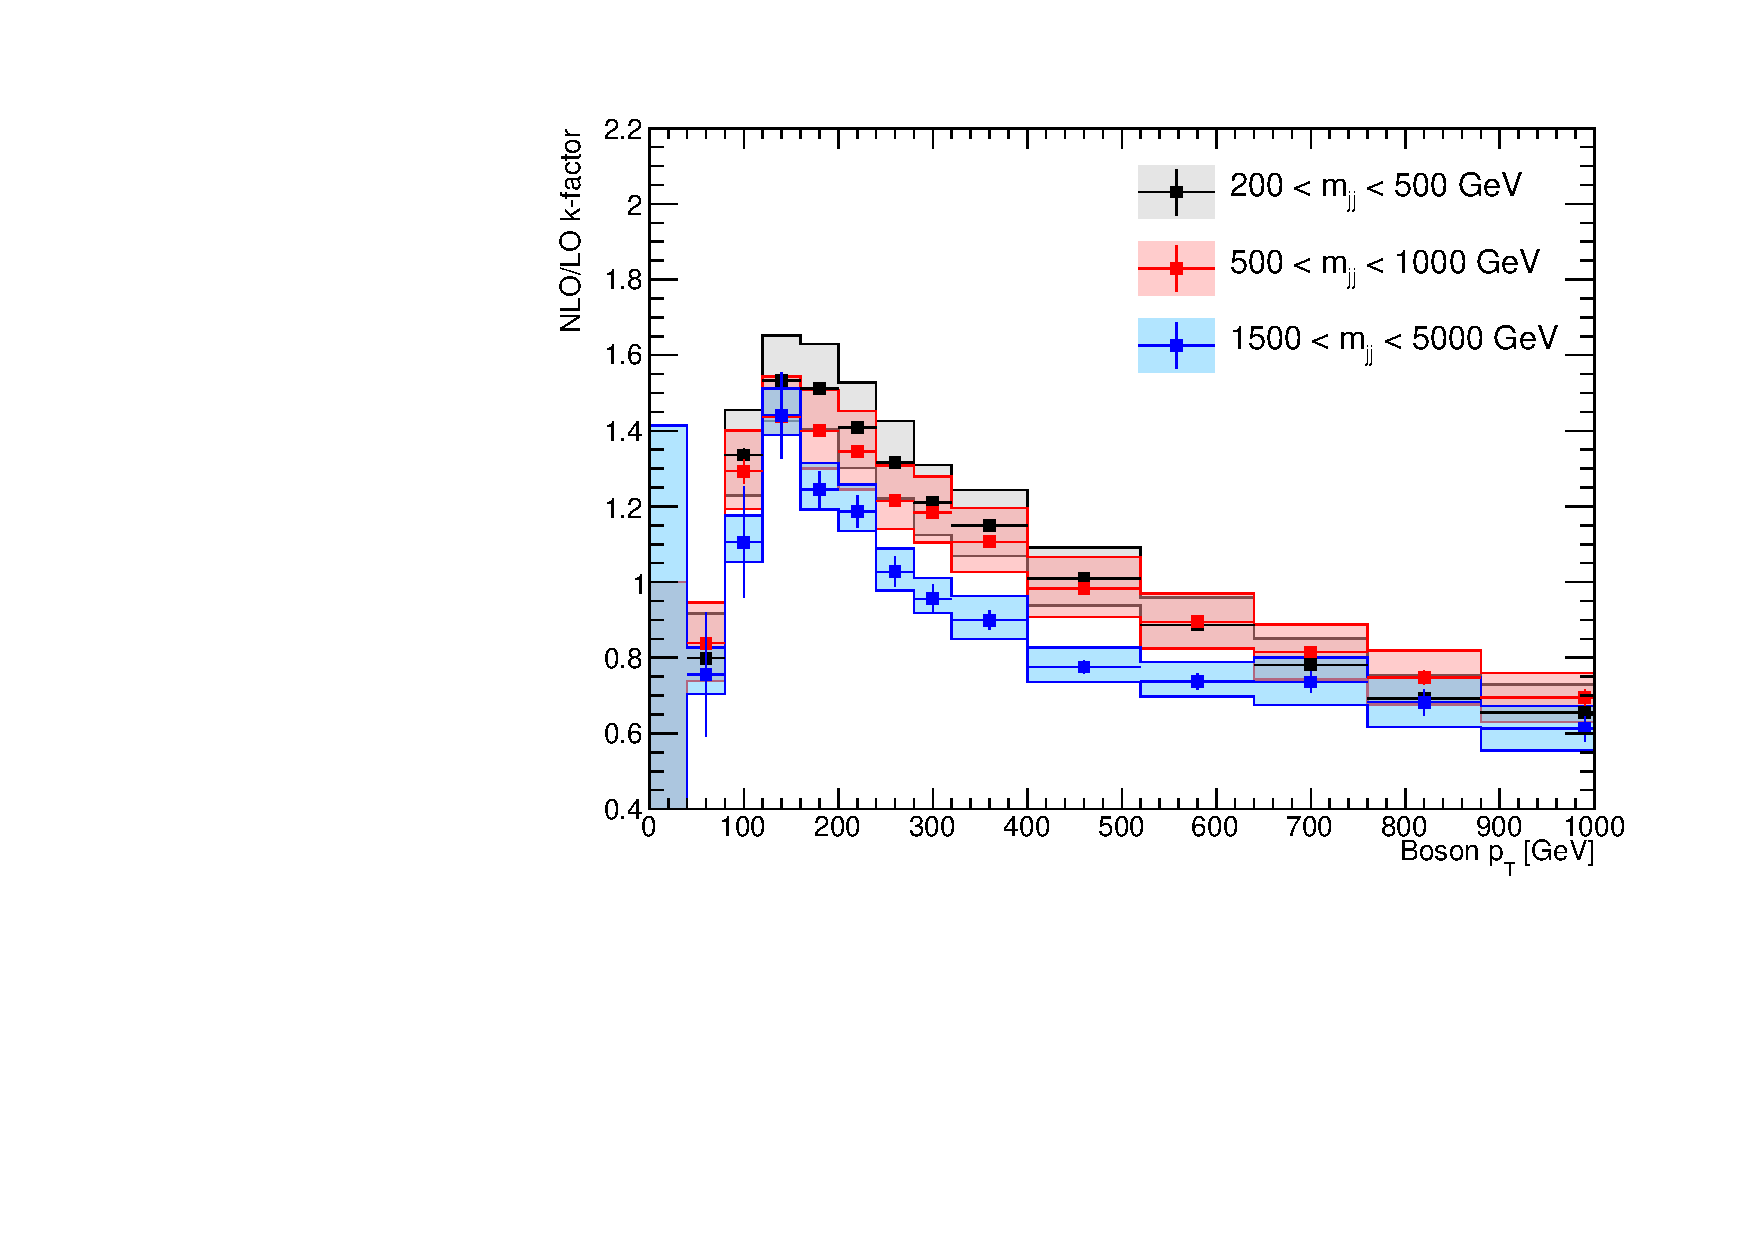
\includegraphics[width=0.49\textwidth]{Objects/kfactor_VBF_zjet_born_default.pdf}
        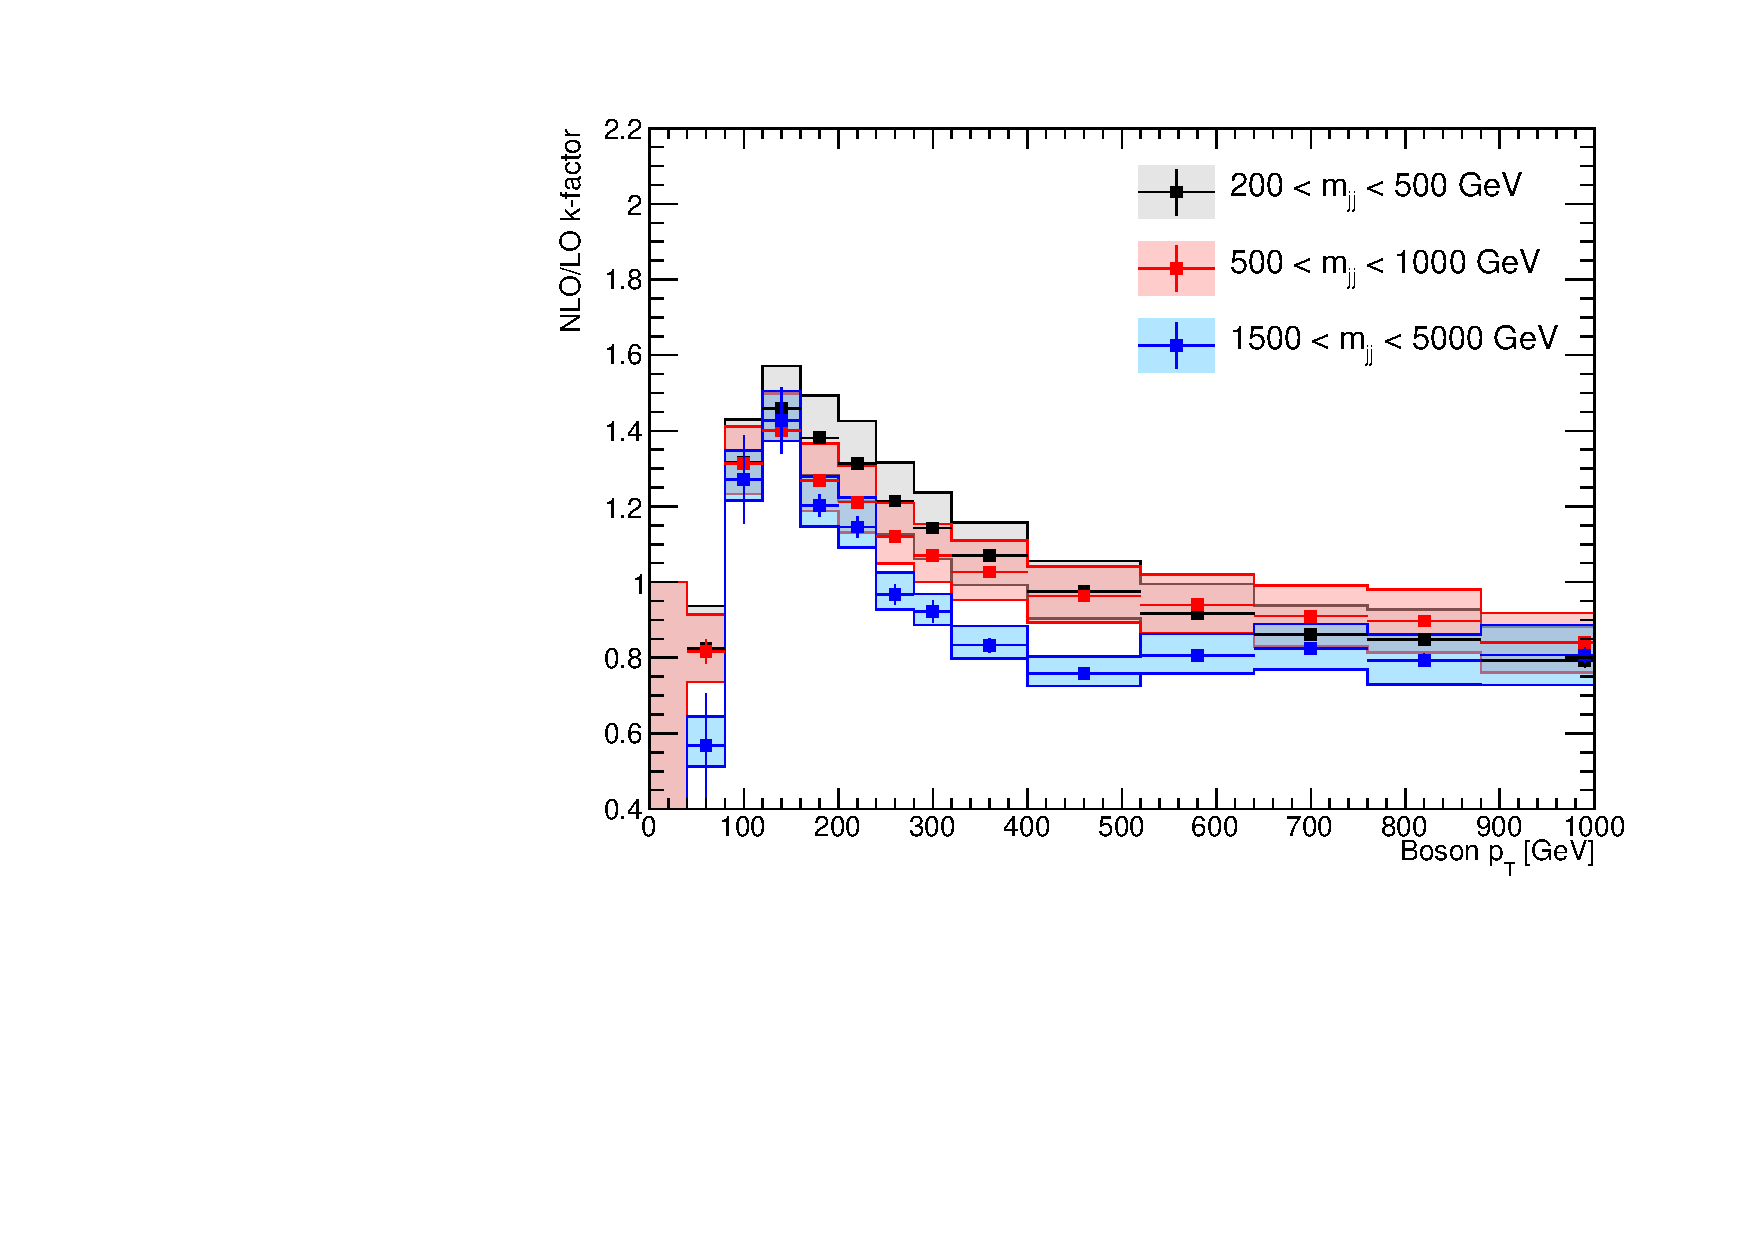
\includegraphics[width=0.49\textwidth]{Objects/kfactor_VBF_wjet_born_default.pdf} \\
        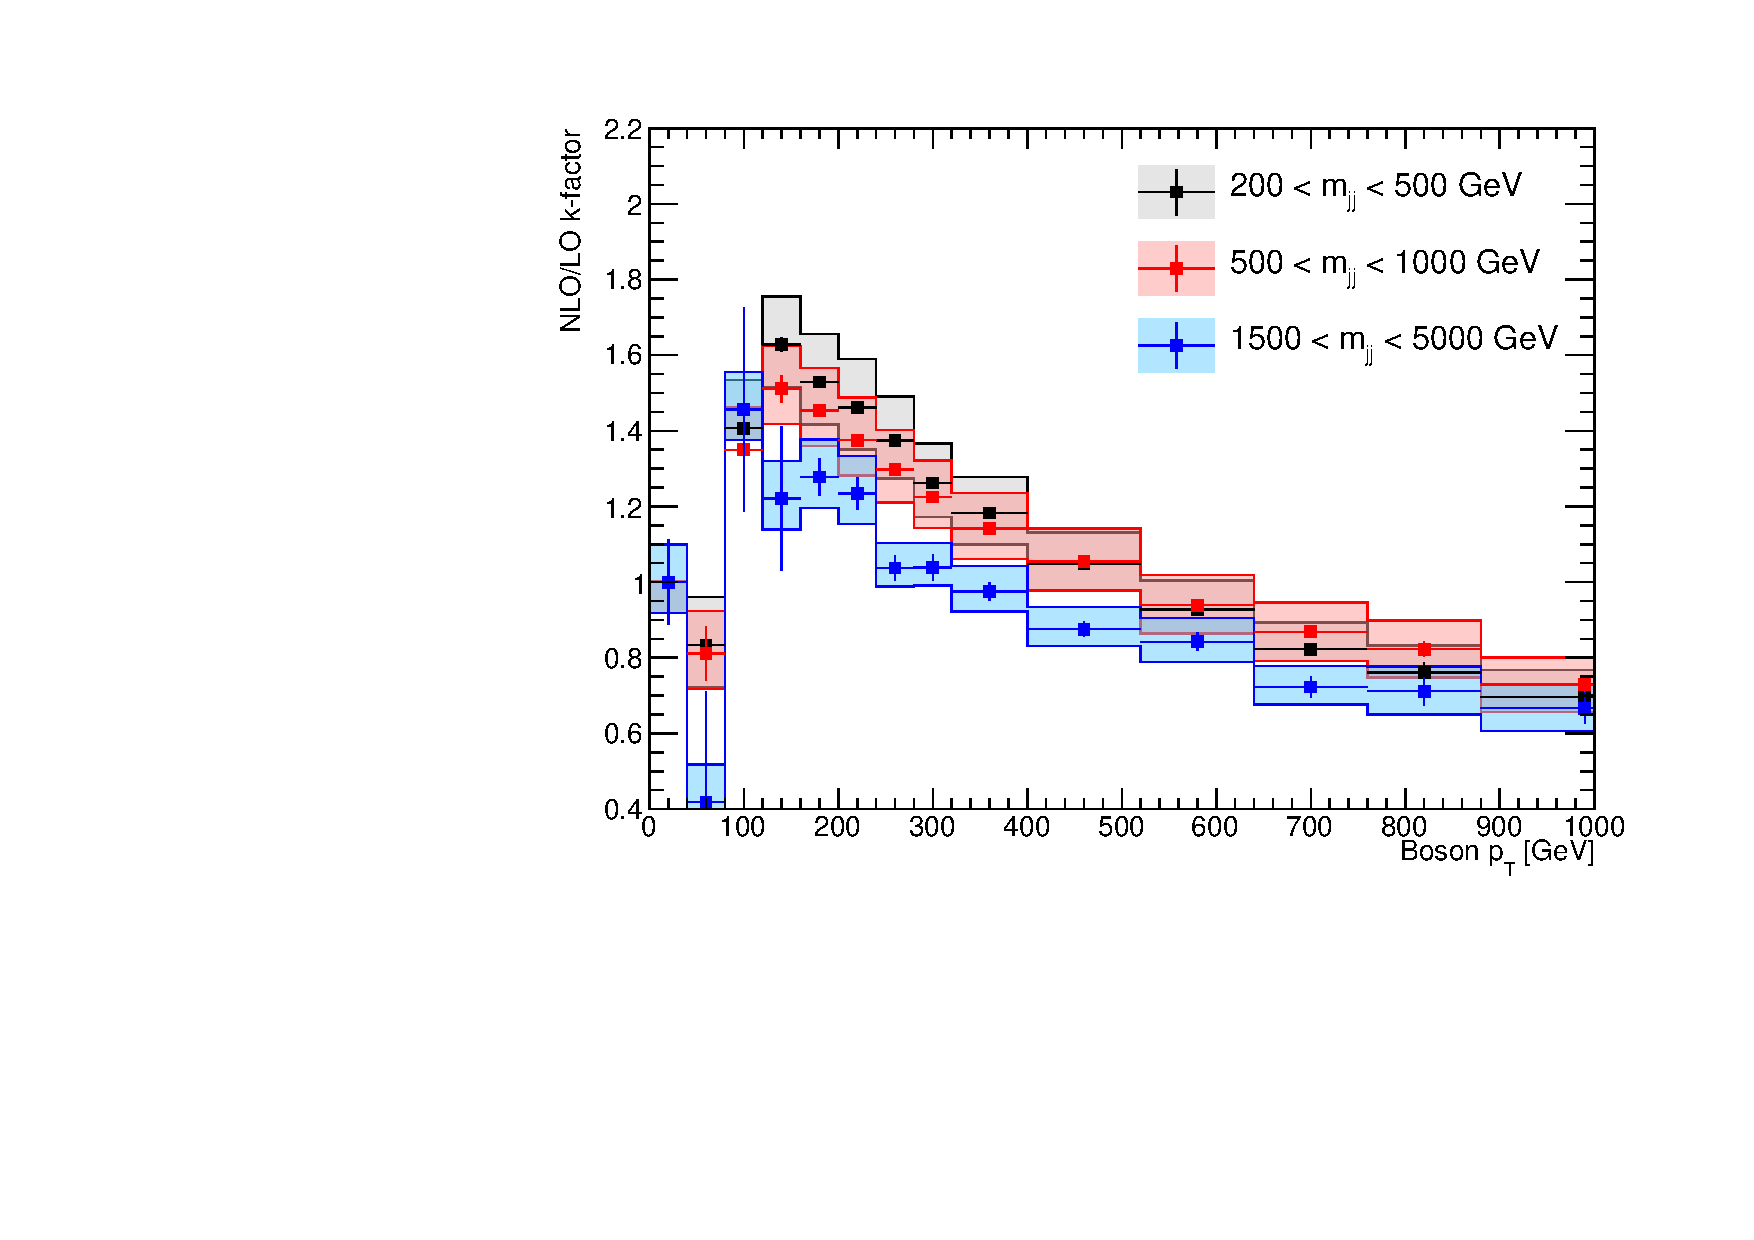
\includegraphics[width=0.49\textwidth]{Objects/kfactor_VBF_znn_born_default.pdf}
        \caption{
            The LO-to-NLO theory scale factors binned in the generator level $p_T^V$ and $m_{jj}$, shown for QCD V+jets processes.
            The scale factors are derived within the generator level selection requirements equivalent to the ones used to form the analysis category defined in Section~\ref{subsec:vbfselection}. The error bars reflect the statistical uncertainty on the bin, while the bands represent the total systematic uncertainty~\cite{note:AN_19_257}.}
      \label{fig:theory_sf_qcd_nlo_2d}
    \end{center}
  \end{figure}
  
  \begin{figure}[htbp]
    \centering
        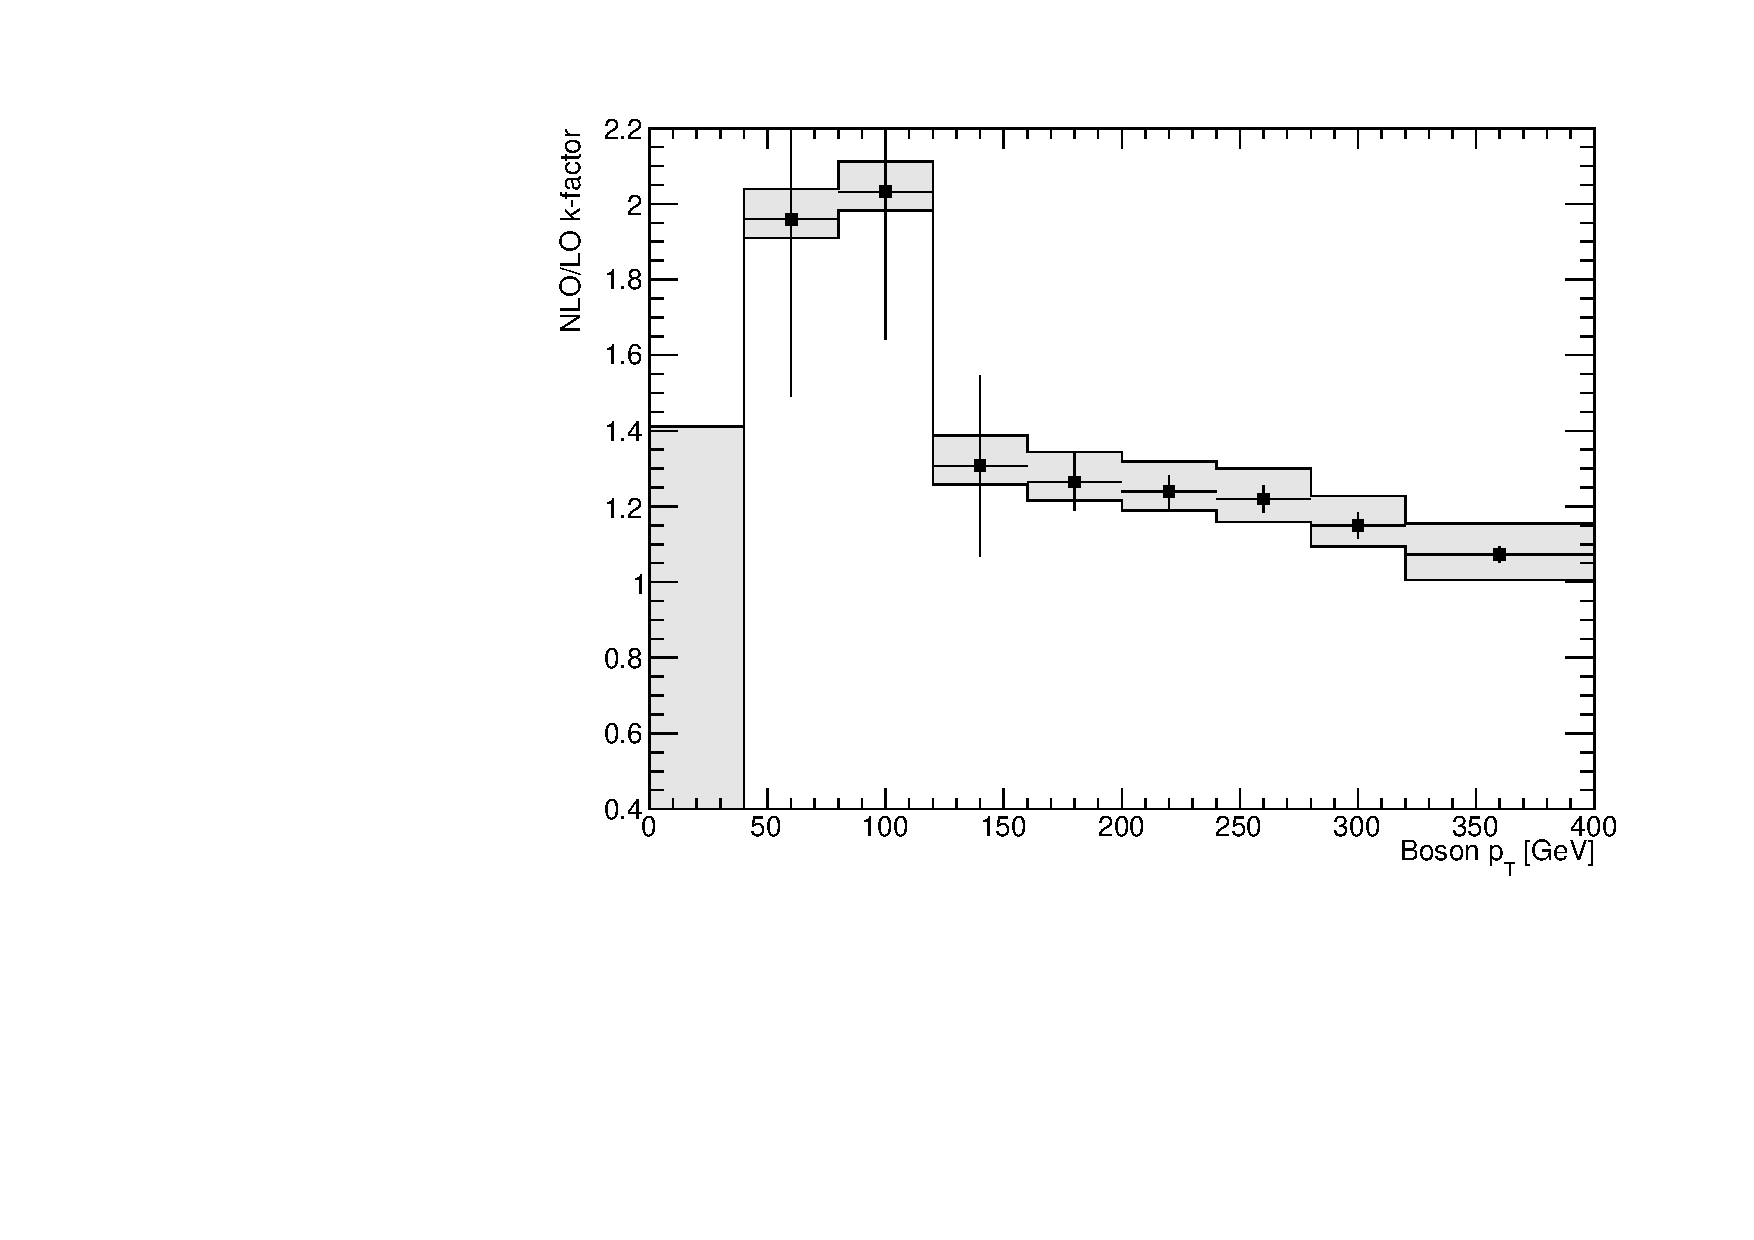
\includegraphics[width=0.45\textwidth]{Objects/kfactor_VTR_zjet_born_default.pdf}
        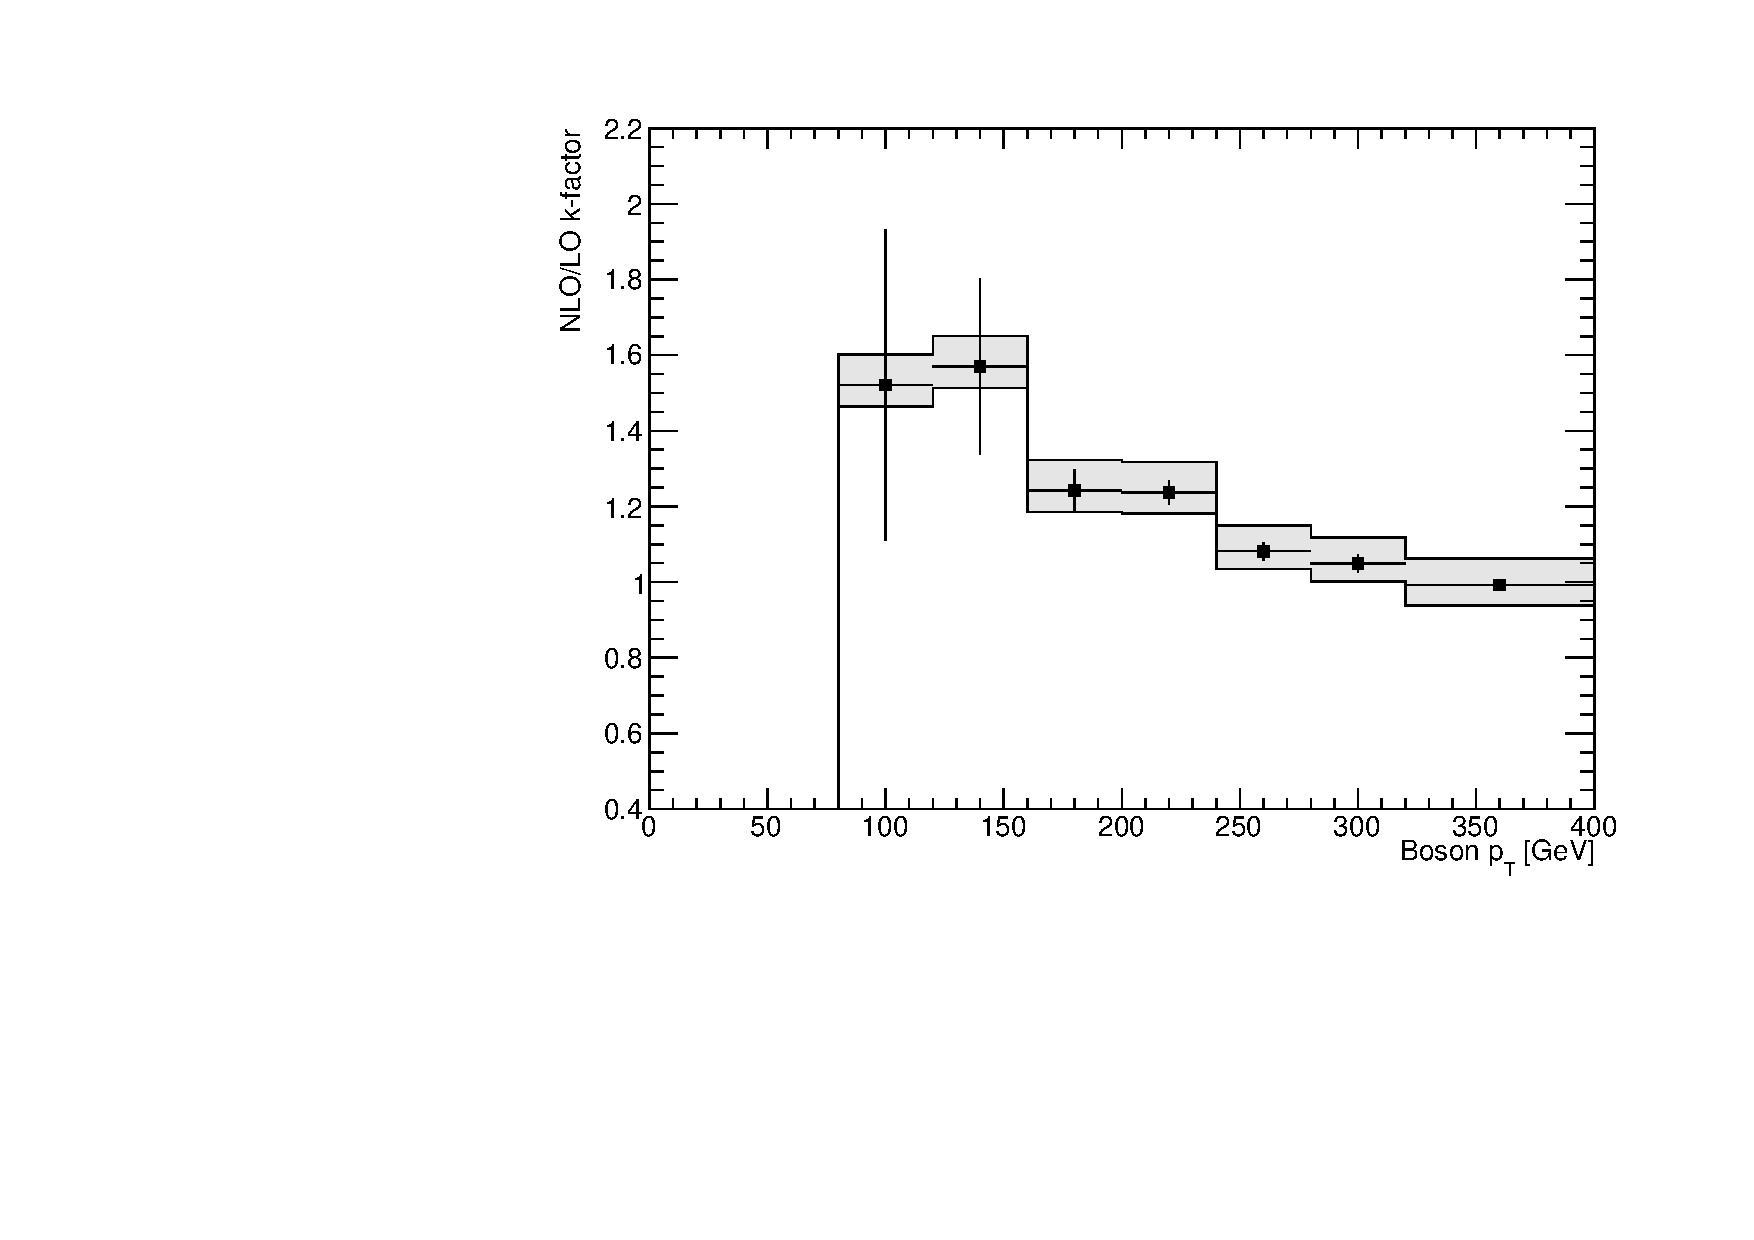
\includegraphics[width=0.45\textwidth]{Objects/kfactor_VTR_wjet_born_default.pdf}\\
        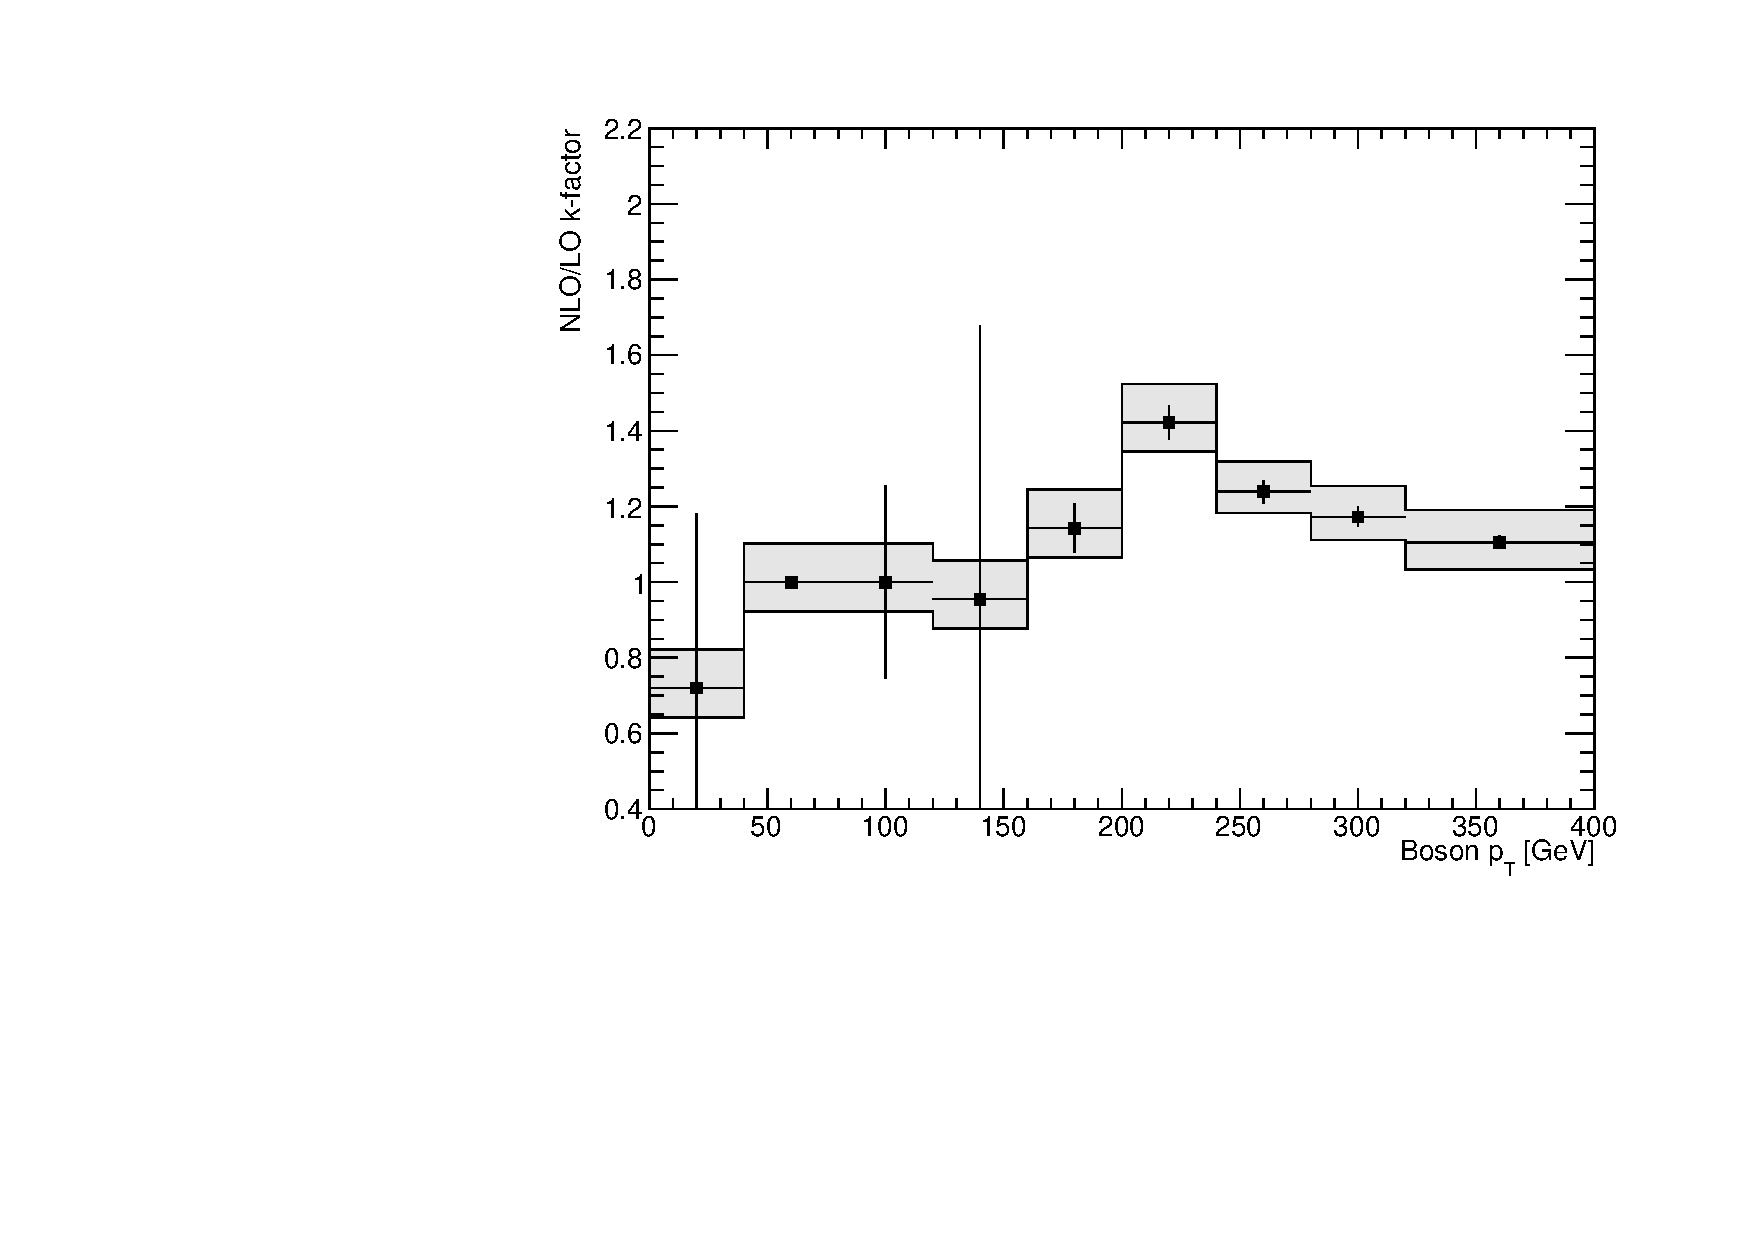
\includegraphics[width=0.45\textwidth]{Objects/kfactor_VTR_znn_born_default.pdf}
    \caption{The LO-to-NLO theory scale factors binned in generator level $p_T^V$, shown for QCD V+jets processes.
            The scale factors are derived within the generator level selection requirements equivalent to the ones used to form the analysis category defined in Section~\ref{subsec:vtr_selection}. The error bars reflect the statistical uncertainty on the bin, while the bands represent the total systematic uncertainty~\cite{note:AN_19_257}.}
    \label{fig:nlo-kfactors-w_n_z-vbf-vtr}
\end{figure}
\hspace{10pt} A similar approach is taken when applying the EWK corrections for QCD V+jets processes. A special ($p_T^{V}$, generator $m_{jj}$) weight map is derived through the application of an equivalent generator level selection as the one used above. Finally, these weights are all applied on an event by event basis~\cite{note:AN_19_257}.